
\begin{itemize}
	\item To characterize terrestrial ecosystem (vegetation and soil) responses and feedbacks resulting from SAI, we analyzed an ensemble of global coupled ESM climate change simulations.
	\item The simulations employed the Community Earth System Model (CESM) and were performed for the Stratospheric Aerosol Geoengineering Large Ensembe (GLENS) project at the National Center for Atmospheric Research (NCAR).
	\item The ensemble simulations followed the Fifth Phase Coupled Model Intercomparison Project (CMIP5) Historical and RCP8.5 simulations from 1850--2100.
	\item The baseline experiment period, called \textbf{\textit{BASE}}, ran for 2010--2019, and the control, called \textbf{\textit{CTRL}}, ran for 2020--2097, following the standard CMIP6 protocol.
	\item A third set of ensemble members, called \textbf{\textit{GEOENG}}, ran for 2020-2097 with simulated SAI mitigation designed to stabilize global temperatures at those for the year 2020.

\end{itemize}


\begin{figure}
	\begin{center}
		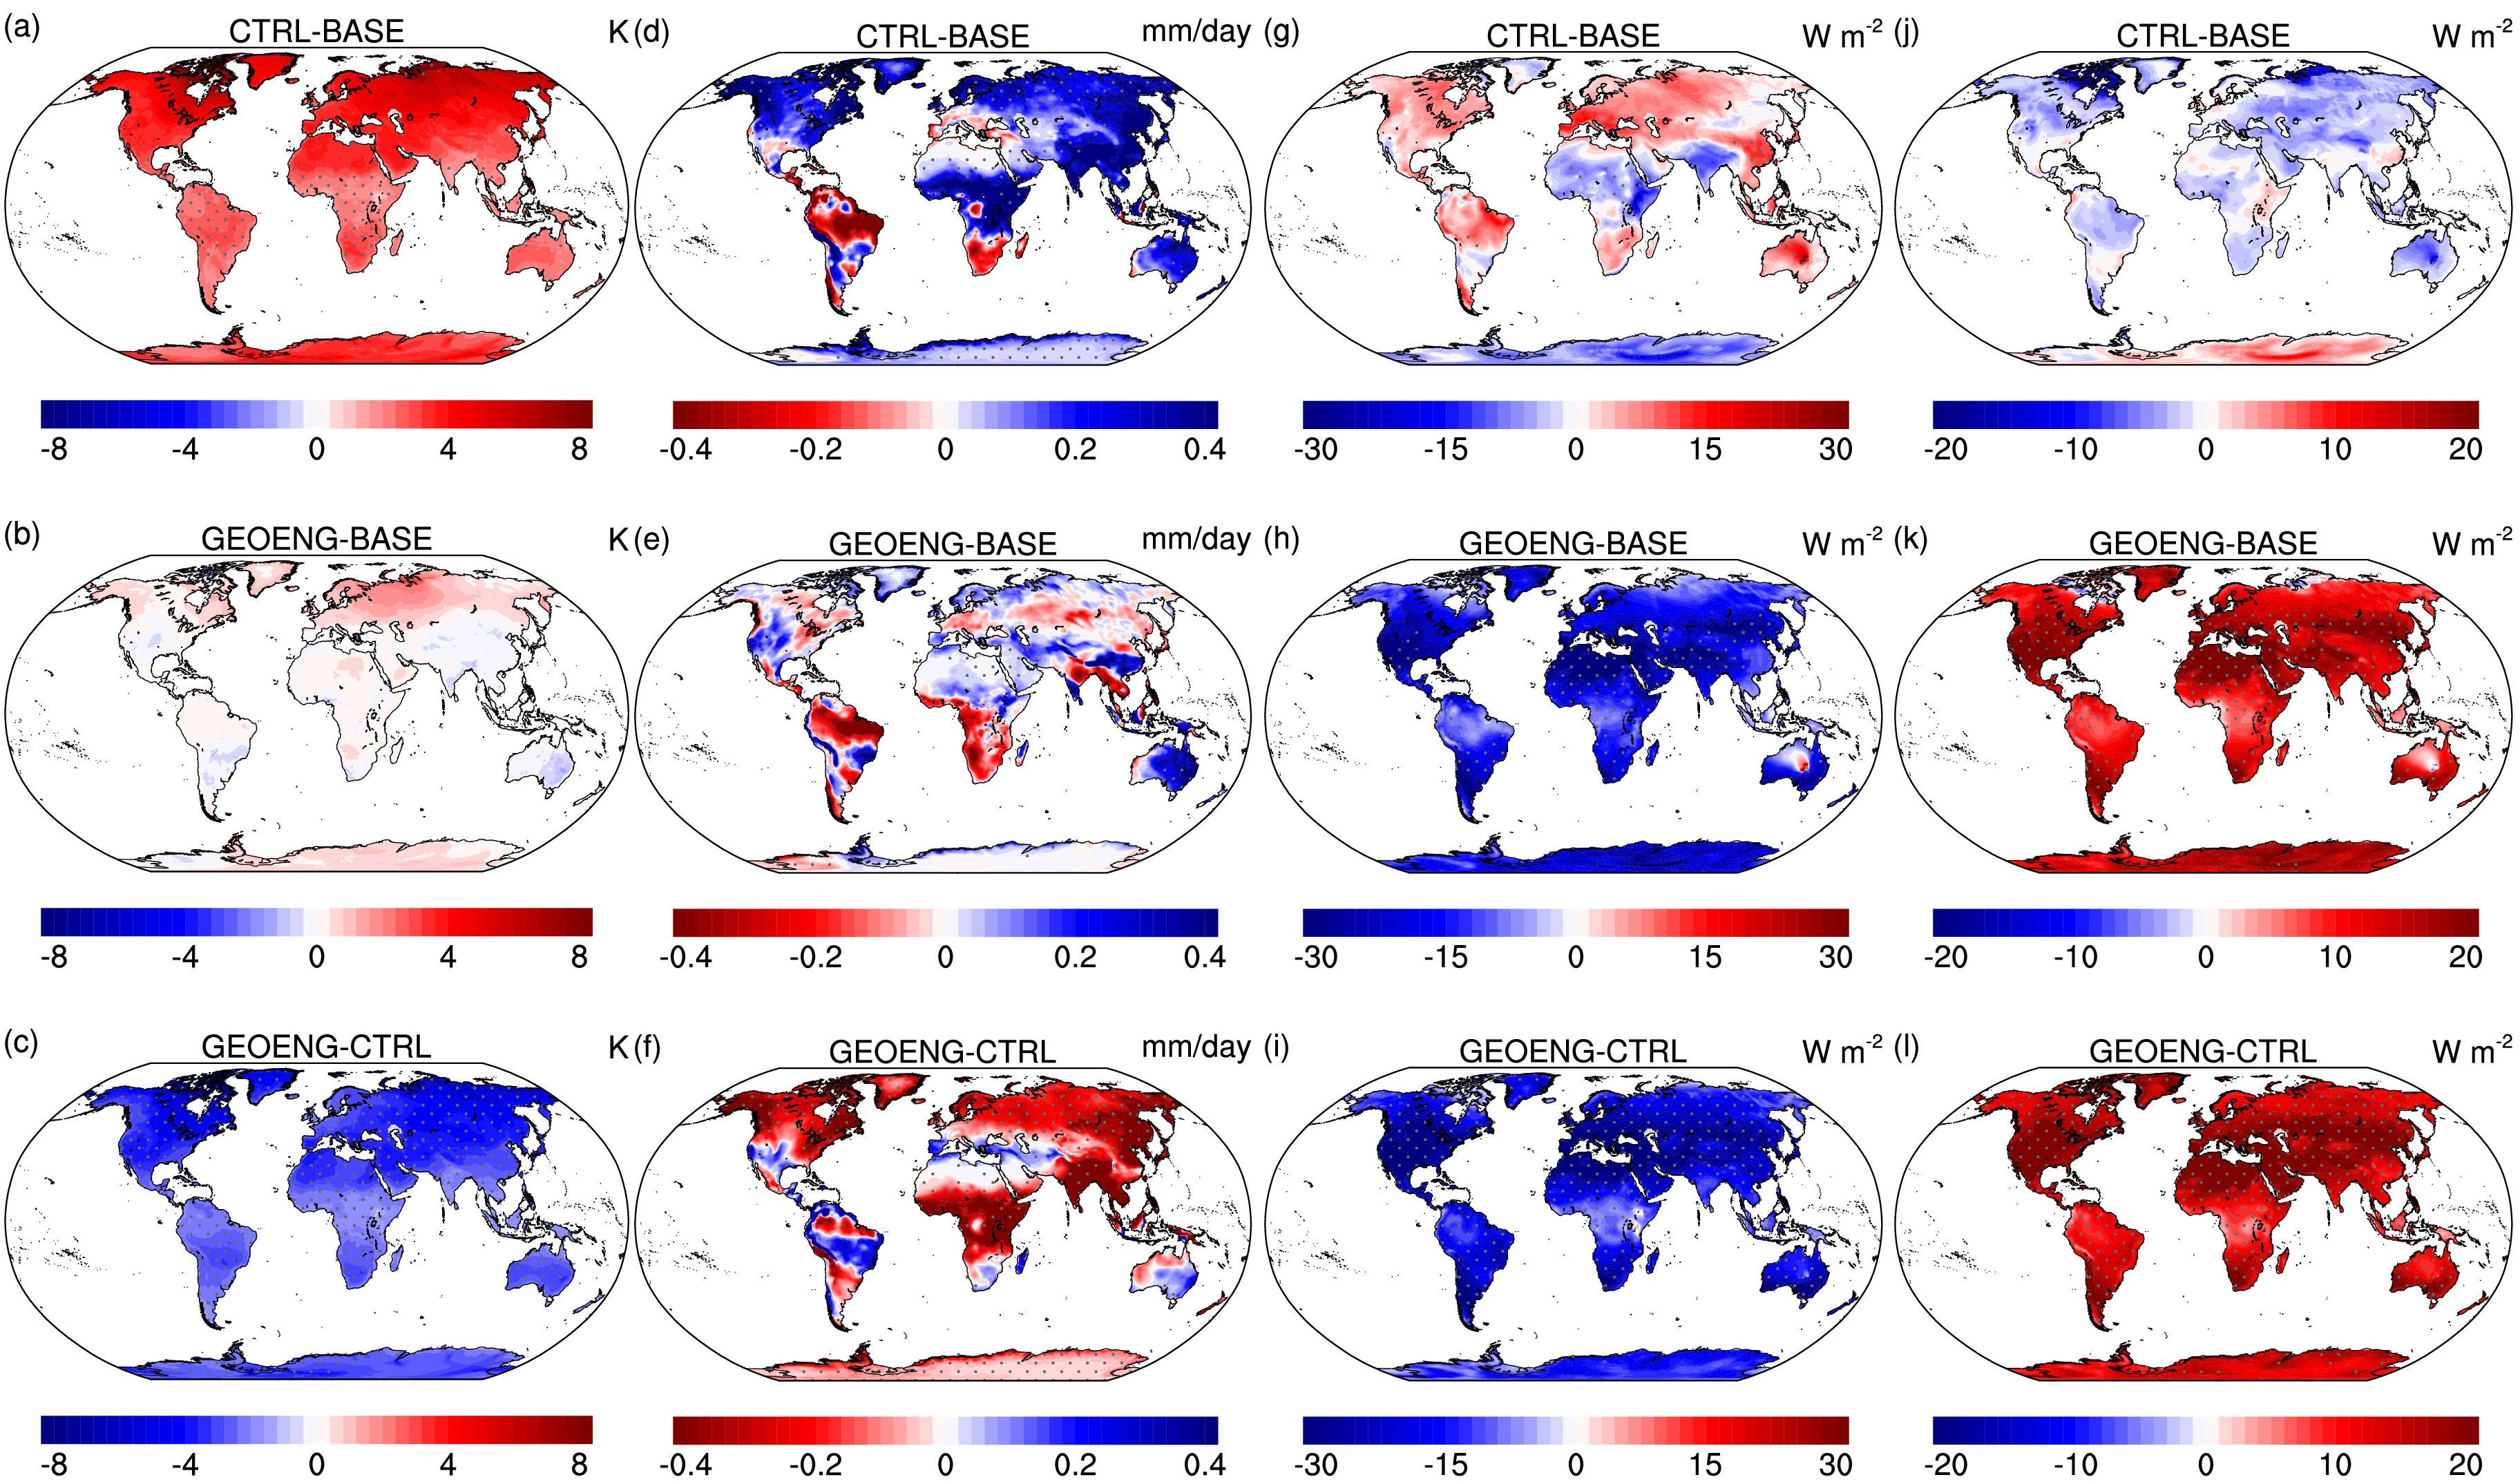
\includegraphics[width=\columnwidth]{erl_figures/Fig2.jpg}
	\end{center}
	\caption{Changes of spatial distributions between CTRL and BASE (top row), between GEOENG and BASE (middle row), and between GEOENG and CTRL (bottom row) for surface temperature (K, (a)--(c)), precipitation (mm\,day$^{-1}$, (d)--(f)), total downward direct solar radiation at the surface (W\,m$^{-2}$, (g)--(i)), and total downward diffuse solar radiation at the surface (W\,m$^{-2}$, (j)--(l)). The spatial distribution of CTRL is from the 2020--2097 time-averaged results without geoengineering while that of GEOENG is from the 2020--2097 time-averaged results with geoengineering applied. The spatial distribution of BASE is from the 2010--2019 time-average results. Light grey stippling (dots) indicates regions where the change is significant using the Student's t-test ($p < 0.1$).
		% https://iopscience.iop.org/article/10.1088/1748-9326/abacf7
	}\label{fig:geoeng_climate}
\end{figure}

\begin{itemize}
	\item Differences in climate variables (surface temperature, precipitation, and downward direct and diffuse solar radiation at the surface) were evaluated (Figure~\ref{fig:geoeng_climate}).
	\item Similarly, differences in terrestrial productivity variables (photosynthesis rate, gross primary production, net primary production, and net biome production) were assessed to characterize responses and feedbacks of the SAI treatment (Figure~\ref{fig:geoeng_bgc}).
\end{itemize}


\begin{figure}
	\begin{center}
		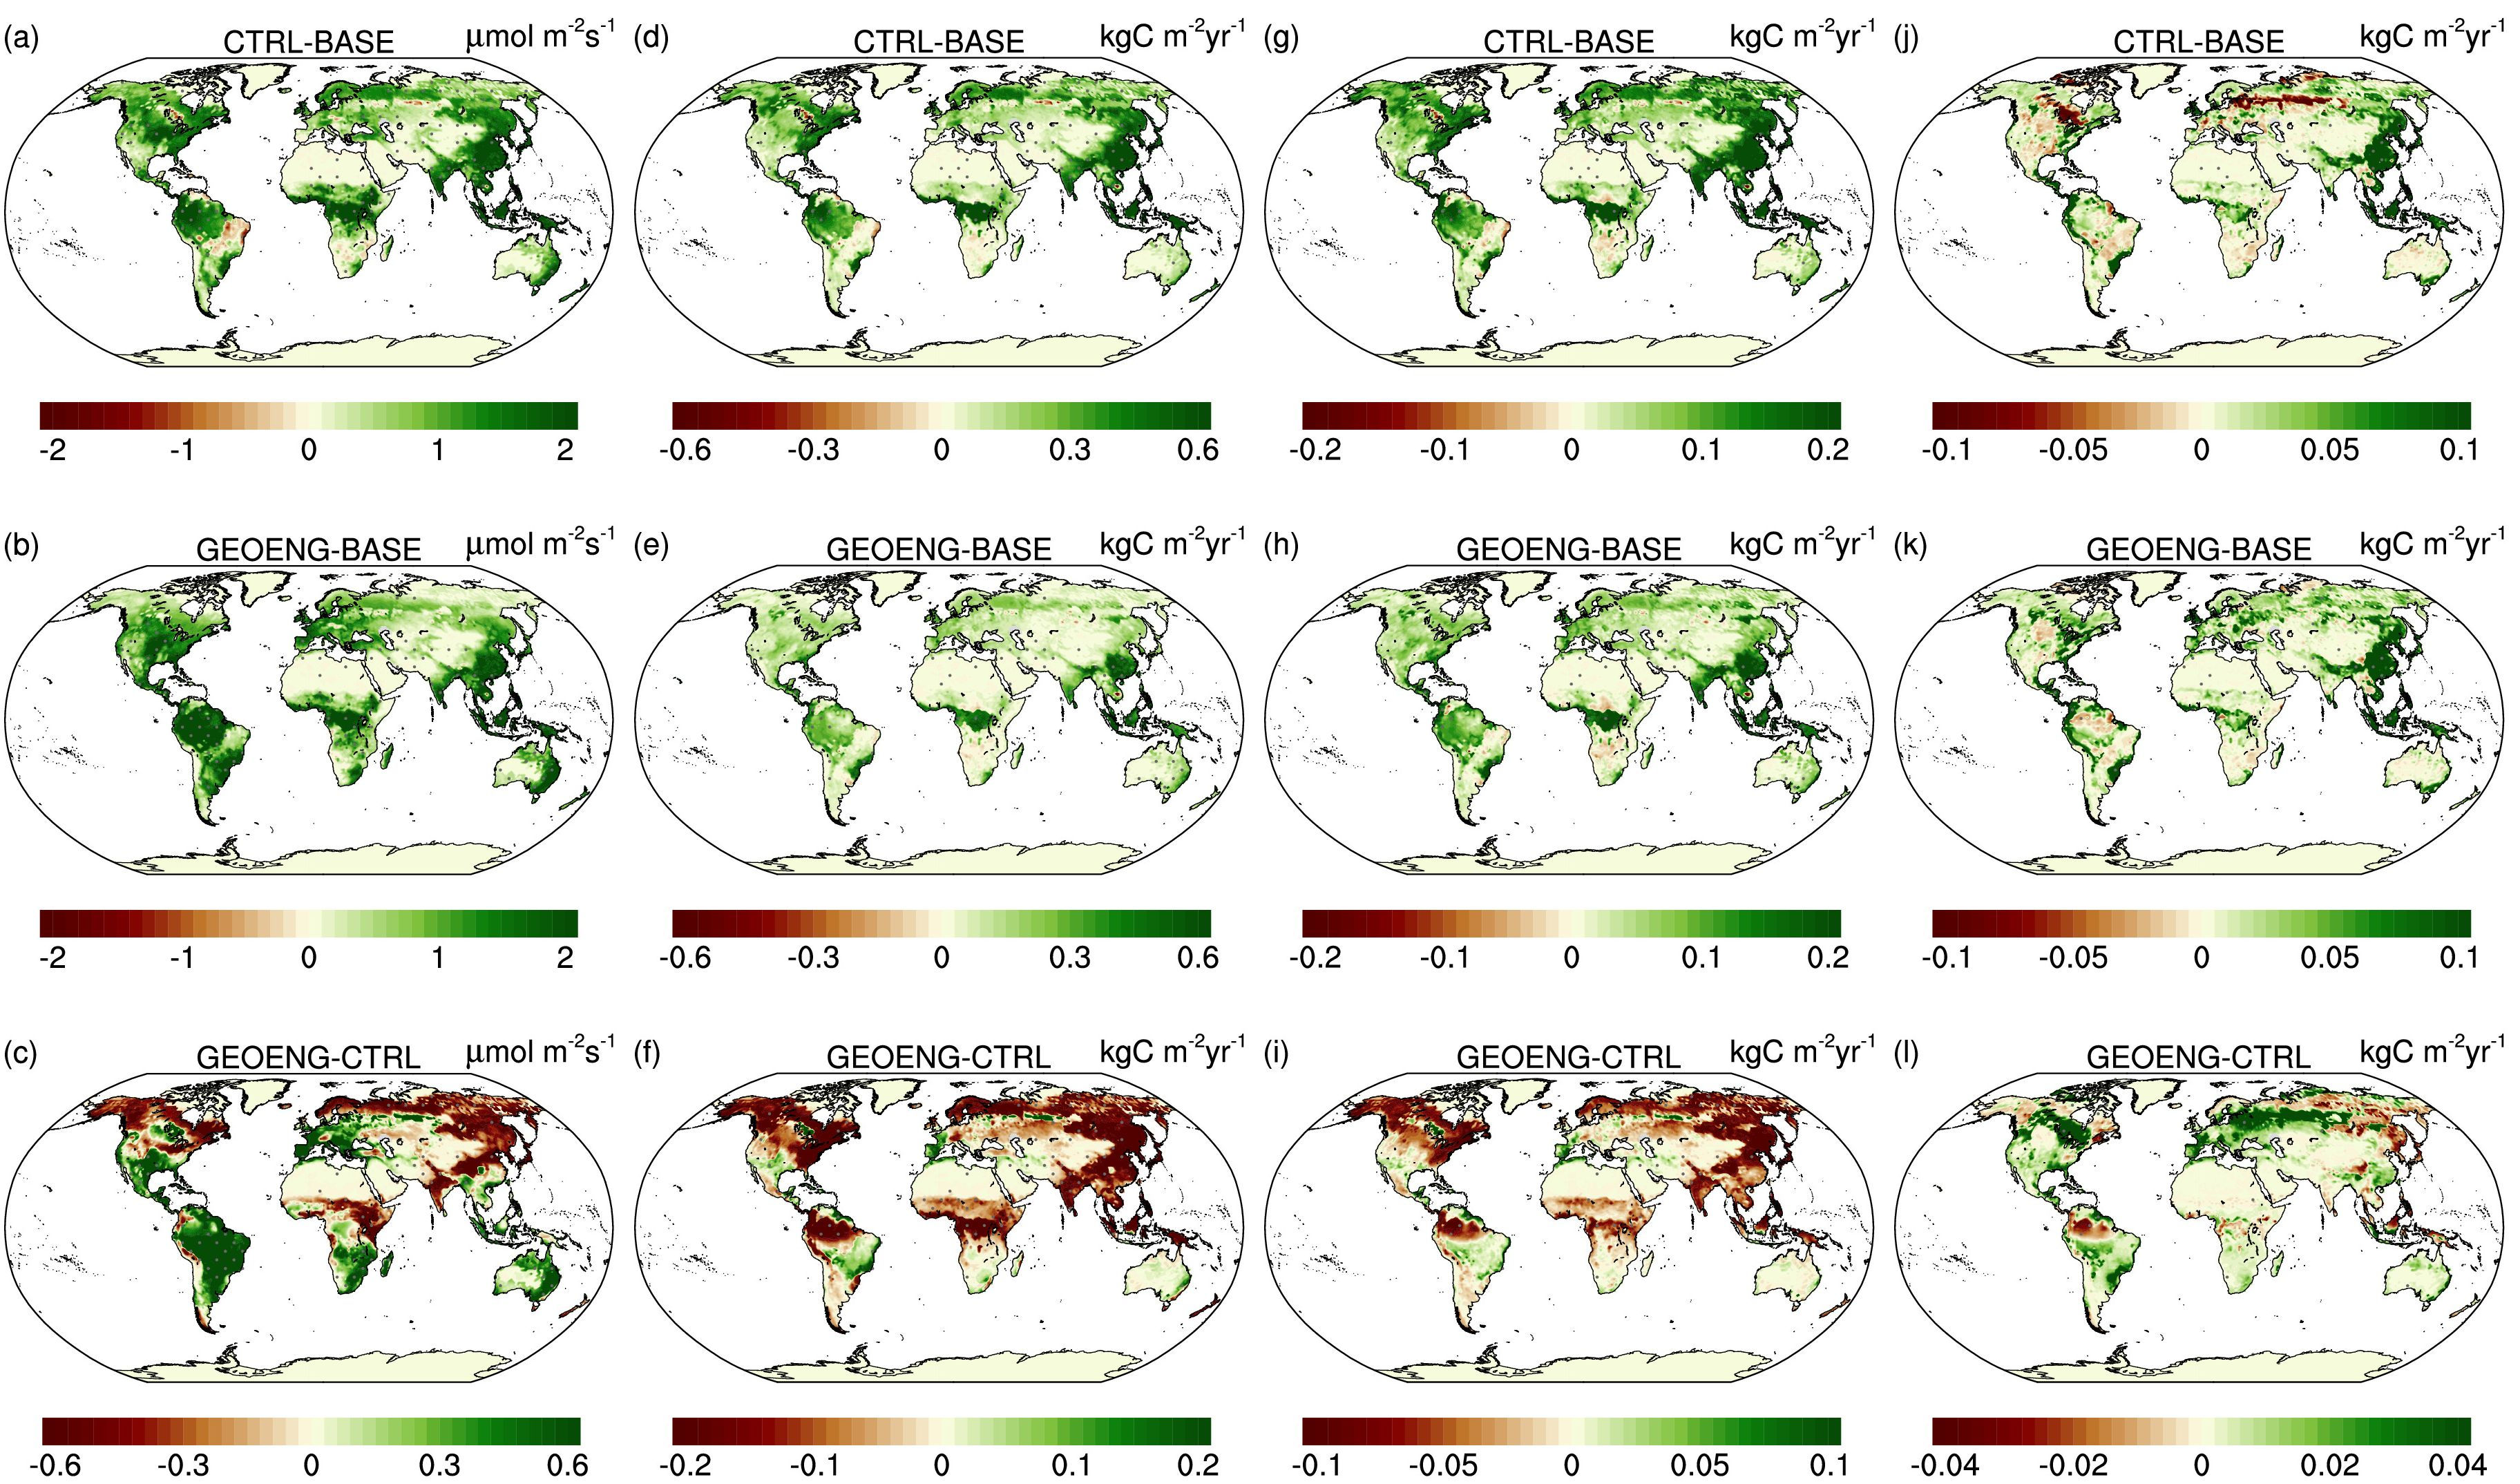
\includegraphics[width=\columnwidth]{erl_figures/Fig3.jpg}
	\end{center}
	\caption{Changes of spatial distributions between CTRL and BASE (top row), between GEOENG and BASE (middle row), and between GEOENG and CTRL (bottom row) for photosynthesis rates (µmol\,m$^{-2}$\,s$^{-1}$, (a)--(c)), gross primary production (kg\,C\,m$^{-2}$\,yr$^{-1}$, (d)--(f)), net primary production (kg\,C\,m$^{-2}$\,yr$^{-1}$, (g)--(i)), and net biome production (kg\,C\,m$^{-2}$\,yr$^{-1}$, (j)--(l)). The spatial distribution of CTRL is from the 2020--2097 time-averaged results without geoengineering while that of GEOENG is from the 2020--2097 time-averaged results with geoengineering applied. The spatial distribution of BASE is from the 2010--2019 time-average results. Light grey stippling (dots) indicates regions where the change is significant using the Student's t-test ($p < 0.1$).
		% https://iopscience.iop.org/article/10.1088/1748-9326/abacf7
	}\label{fig:geoeng_bgc}
\end{figure}


\begin{itemize}
	\item The carbon sink strength on land increased under the SAI geoengineering treatment, accumulating an additional 79\,$\pm$\,6~Pg\,C on land between 2020 and 2097 (Figure~\ref{fig:geoeng_CO2_SO2}a).

	\item If the simulation had been coupled in a way that the atmospheric CO$_2$ trajectory responded to that difference in terrestrial carbon uptake, the atmospheric CO$_2$ mole fraction would have been 872~ppm instead of 909~ppm at the year 2097, absent ocean feedbacks not incorporated into the simulations (Figure~\ref{fig:geoeng_CO2_SO2}b).

	\item Using a simple linear model, we estimated that the additional land carbon sink in the simulation would have lowered surface temperature by about 0.14$^\circ$C at 2097, again assuming no ocean interactions (Figure~\ref{fig:geoeng_CO2_SO2}c).

	\item We further estimated that sulfur injection rates could have been slightly adjusted to instead maintain a constant global temperature (Figure~\ref{fig:geoeng_CO2_SO2}d).
\end{itemize}

\begin{figure}
	\begin{center}
		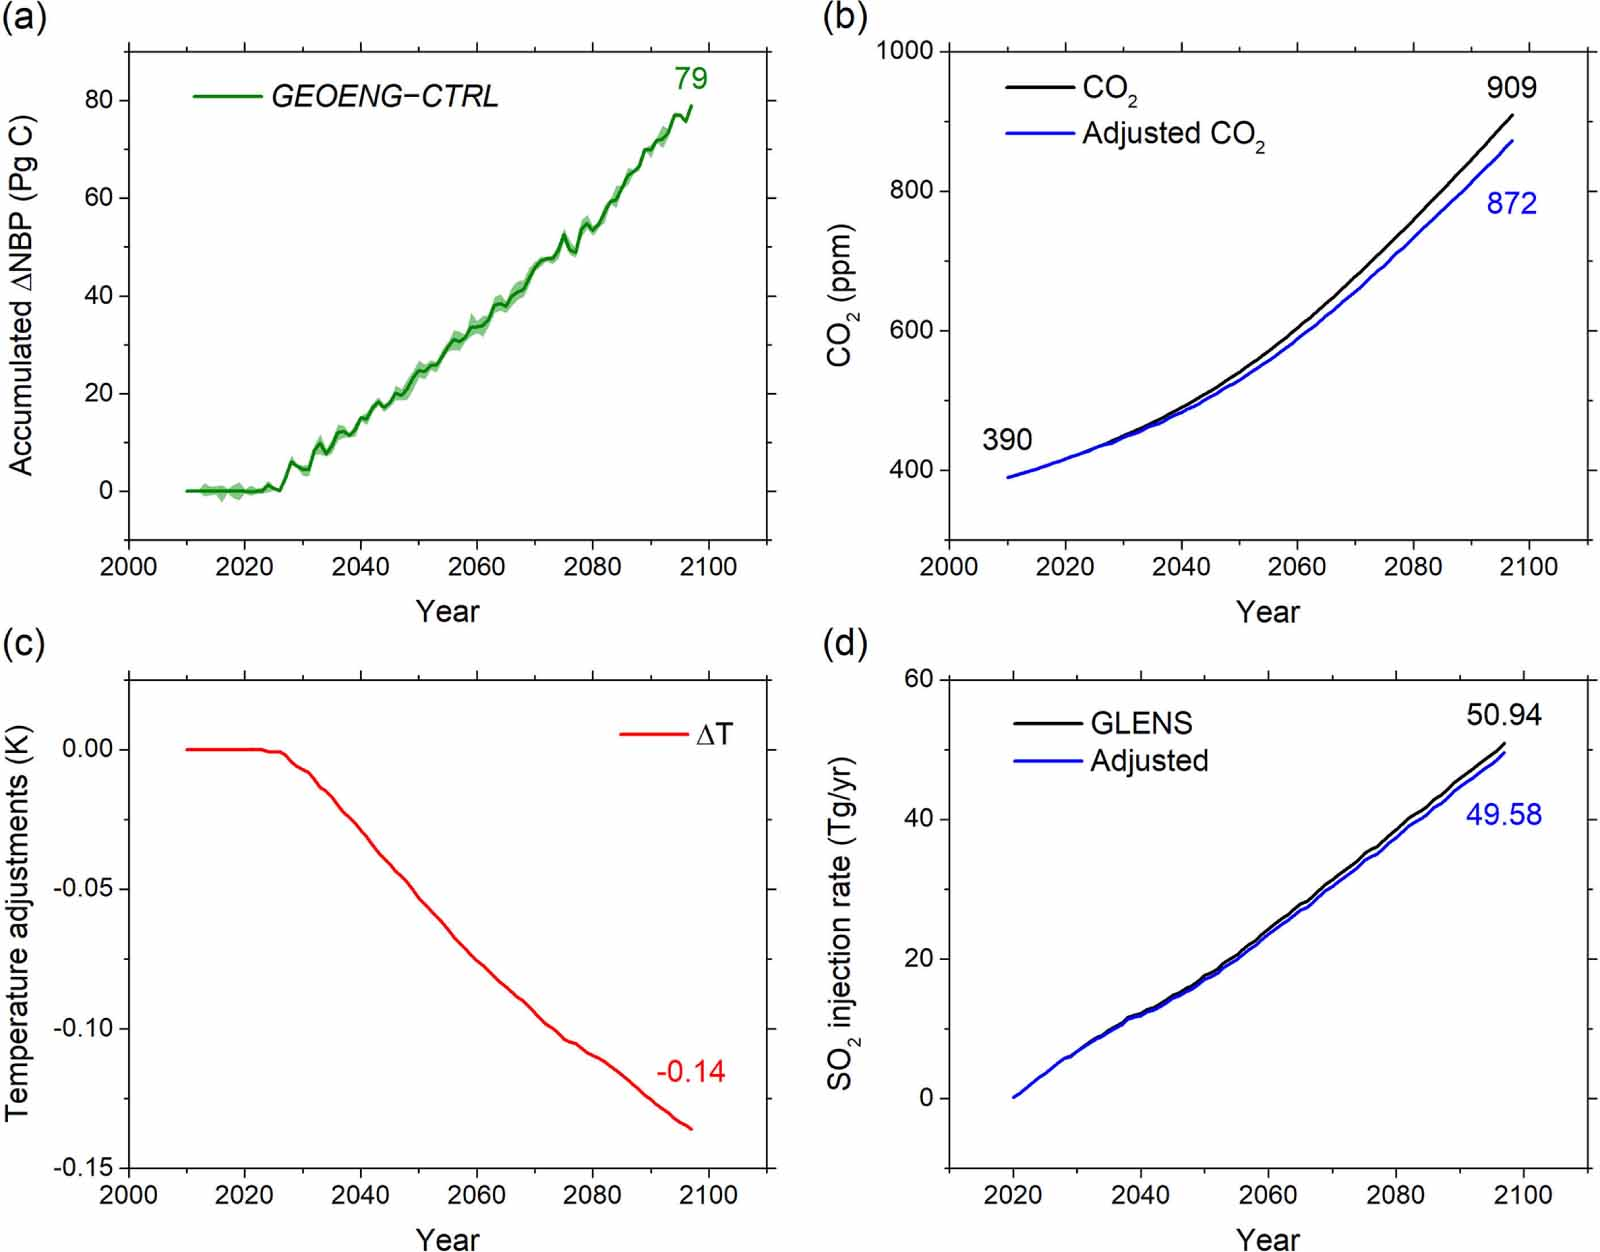
\includegraphics[width=0.85\columnwidth]{erl_figures/Fig4.jpg}
	\end{center}
	\caption{The trajectories of (a) accumulated global carbon sink strength changes (Pg\,C) due to geoengineering, (b) the atmospheric CO$_2$ mole fraction (ppm) during 2010--2097 for BASE+CTRL (black line) and the adjusted atmospheric CO$_2$ mole fraction due to terrestrial BGC feedbacks under geoengineering (blue line), (c) surface temperature responses (K) due to atmospheric CO$_2$ adjustments, and (d) sulfur injection rates (Tg\,yr$^{-1}$) in GLENS (red) and adjusted injection rates due to terrestrial BGC feedbacks (blue).
		% https://iopscience.iop.org/article/10.1088/1748-9326/abacf7
	}\label{fig:geoeng_CO2_SO2}
\end{figure}

\begin{itemize}
	\item This study showed that a geoengineering mitigation strategy with SAI under a high greenhouse gas emission scenario would have increased land carbon storage by 79~Pg\,C globally, primarily as a result of lower ecosystem respiration and diminished disturbance effects under the SAI treatment.

	\item \textbf{Fully coupled emissions-forced simulations with interactive terrestrial and marine biogeochemistry are required to quantify competing feedback effects.}
\end{itemize}
